\documentclass[12pt]{article}
\usepackage[utf8]{inputenc}
\usepackage{graphicx}
\usepackage{pdflscape}
\usepackage{float}
\usepackage{geometry}
\usepackage{hyperref}
\usepackage{indentfirst}
\usepackage[justification=centering,labelfont=bf]{caption}
\usepackage{subcaption}

\title{CS352 Evolutionary Computation: Homework 3}
\author{Ayat Ospanov, Eliot Heinrich}
\date{\today}

\begin{document}

\maketitle

\section{Fitness benchmark}

In this experiment, the efficacy and speed of several variations of CMA-ES and Differential Evolution algorithms are tested for three fitness landscapes and problem sizes. The spherical fitness, the Schwefel fitness, and Rastrigins fitness are benchmarked for $N=\{2,5,10\}$. Figures \ref{fig:sphere}, \ref{fig:schwefel}, and \ref{fig:rastrigin} show the best fitness of each generation plotted against the runtime and the total number of calls to the fitness function. 

From figure \ref{fig:sphere}, it is clear that CMA-ES algorithms very quickly outperform DE, especially for higher dimensions. All six algorithms are able to converge on a solution, but CMA-ES does do many orders of magnitude faster. For the $N=10$ spherical fitness, for example, CMA-ES finds a solution within $10^{-300}$ within the first $10^5$ calls to the fitness function, whereas DE is unable to get this close until $16 \times 10^{5}$ calls.

Figure \ref{fig:schwefel} tells a similar, but even more exaggerated story. CMA-ES very quickly outperforms DE algorithms, even in the $N=2$ case. This is somewhat unsurprising; CMA-ES is designed for problems with high covariance, such as the Schwefel function. 

Figure \ref{fig:rastrigin} shows that the dynamics of Rastrigins function are dramatically different from the spherical and Schwefel fitnesses. CMA-ES converges for a few generations before become trapped. It is then unable to converge on a true solution at all. DE is able to find solutions, albeit significantly slower than for simpler fitness landscapes. Rastrigins function includes many local optima; it seems that CMA-ES is very susceptible to being trapped in these local optima with no way to escape, whereas DE is able to eventually climb out of these traps. 

It seems then that CMA-ES is much faster option for fitness landscapes with fairly simple gradients (no local optima). Evolutionary algorithms across the board struggle with bumpy fitness landscapes, but differential evolution seems to be able to navigate them to some extent, even when CMA-ES fails completely. The path DE takes through Rastrigins function is somewhat odd; the plots show that it becomes trapped around certain fitnesses for long periods of time before eventually escaping. This is especially visible in the $N=10$ problem; the algorithm almost seems to be taking discrete steps through the fitness landscape.




% BEGIN LANDSCAPE PAGE
\begin{landscape}
\thispagestyle{empty}
    \begin{figure}
        \hspace*{-4.5cm}
        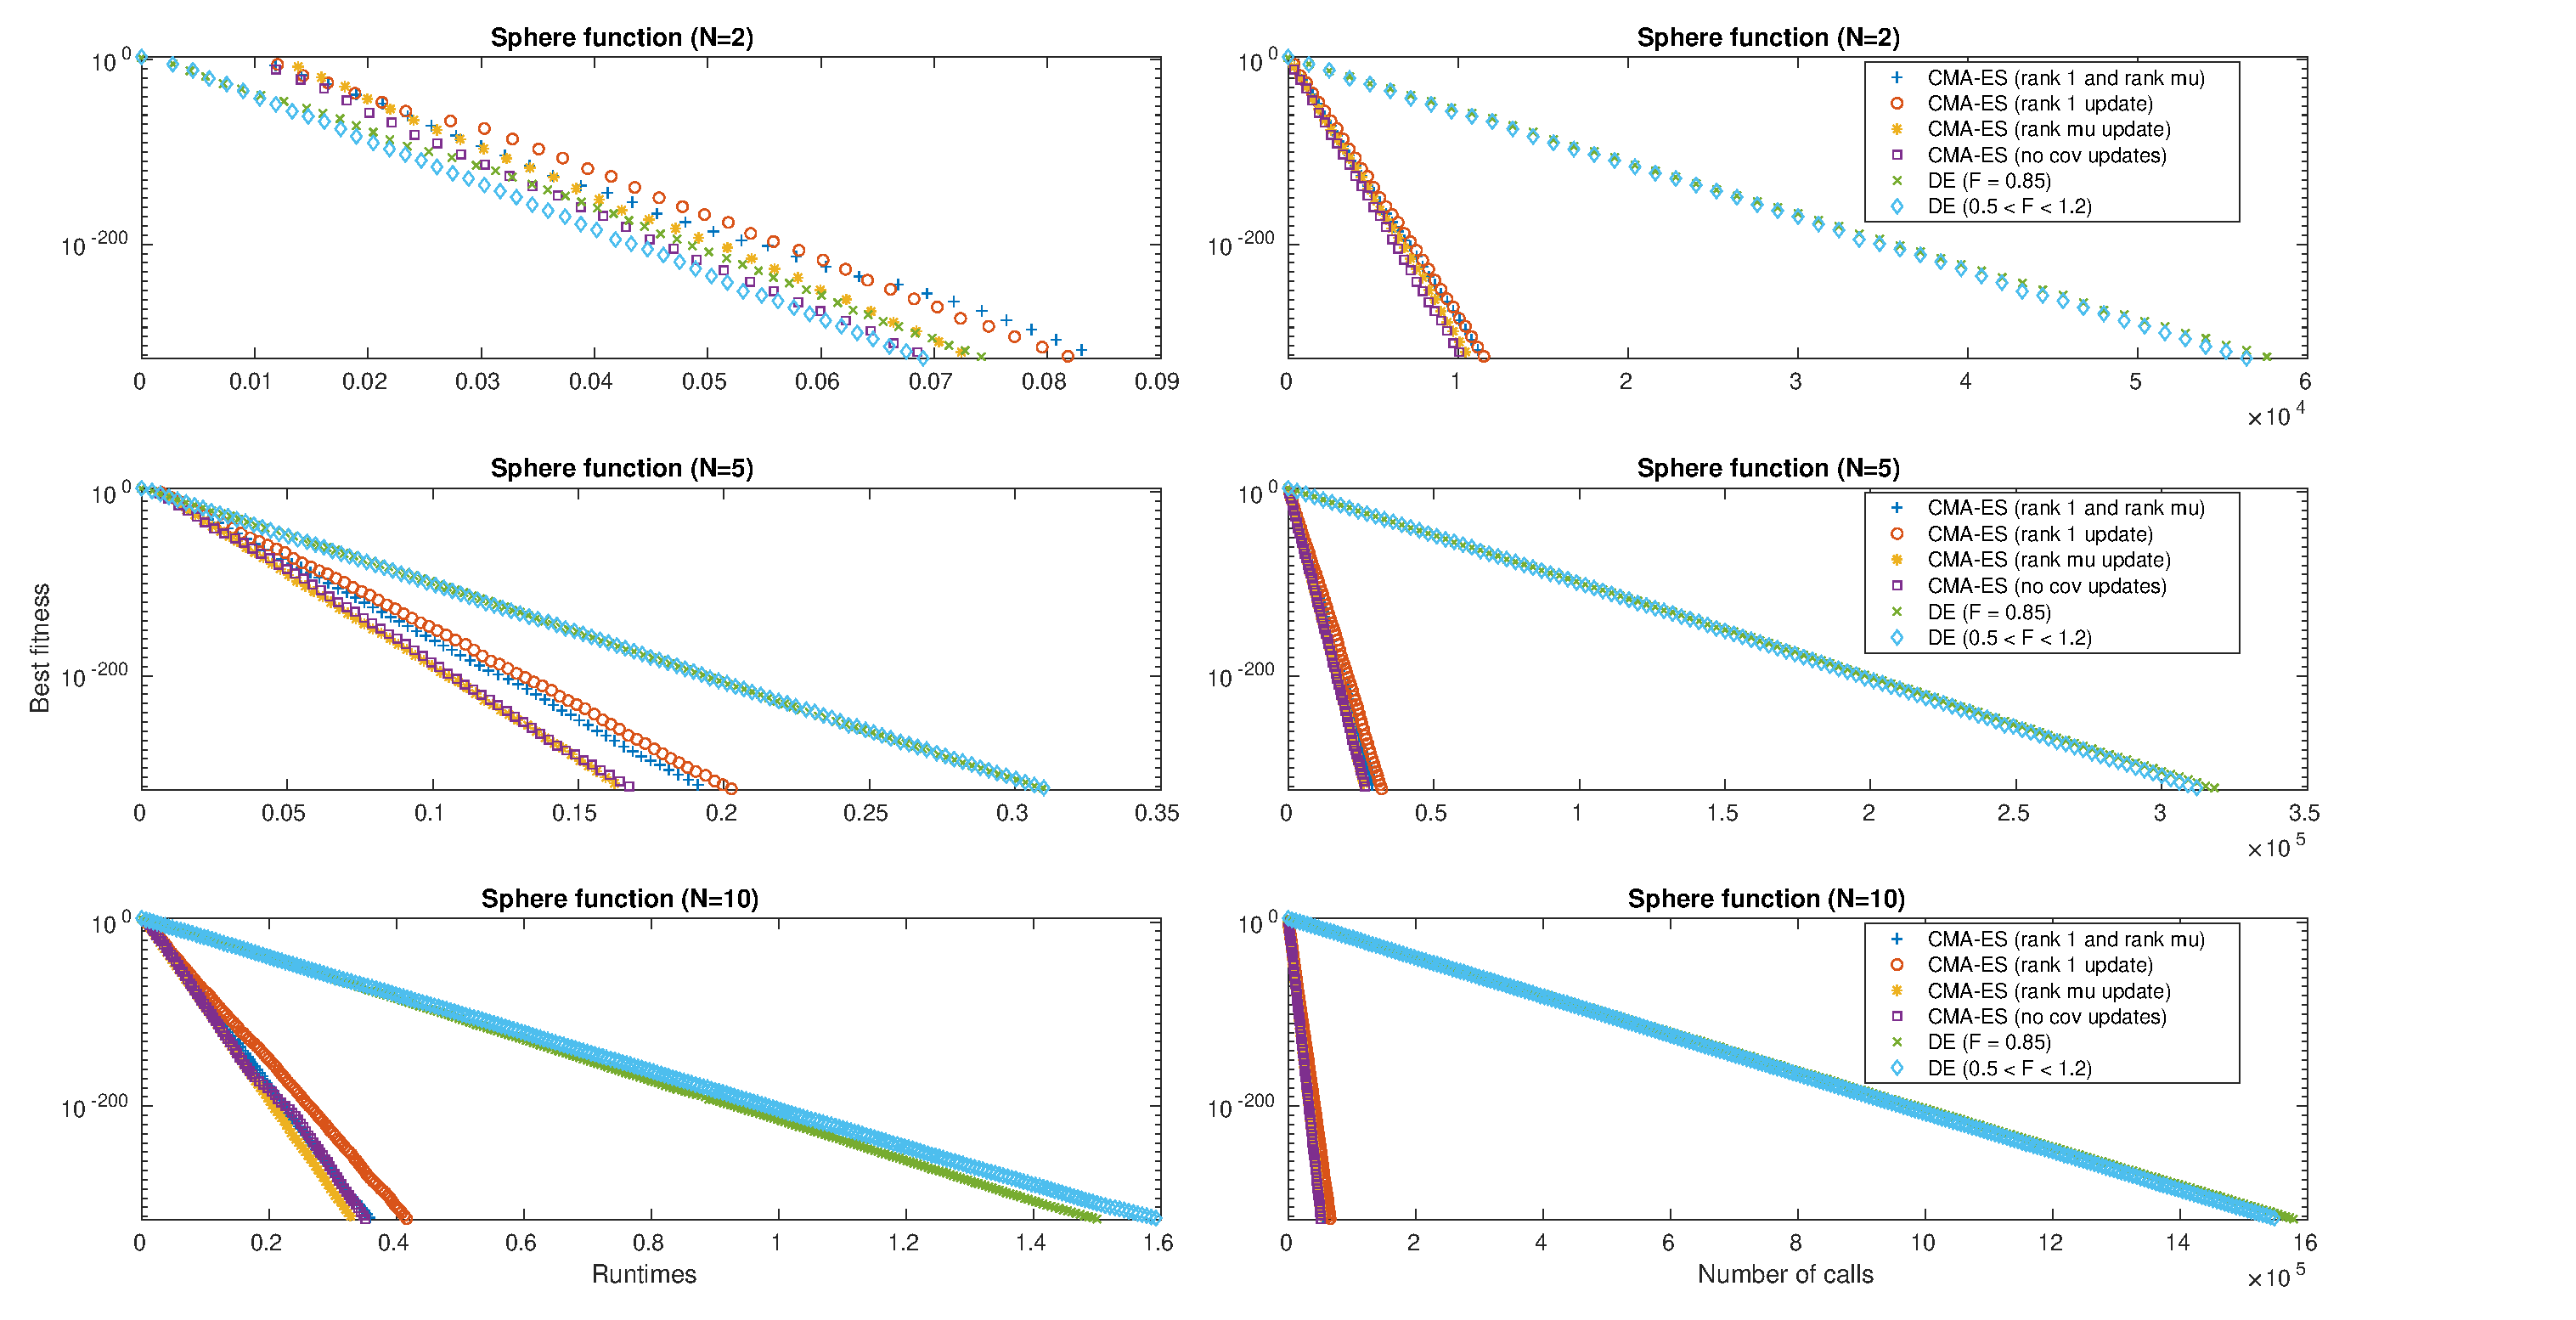
\includegraphics[width=1.5\linewidth]{pics/sphere.eps}
        \caption{Best fitness vs. Runtimes (left column) and
        best fitness vs. Number of calls (right column)
        for the Sphere function (N=\{2,~5,~10\})}
        \label{fig:sphere}
    \end{figure}
\end{landscape}
% END LANDSCAPE PAGE

% BEGIN LANDSCAPE PAGE
\begin{landscape}
\thispagestyle{empty}
    \begin{figure}
        \hspace*{-4.5cm}
        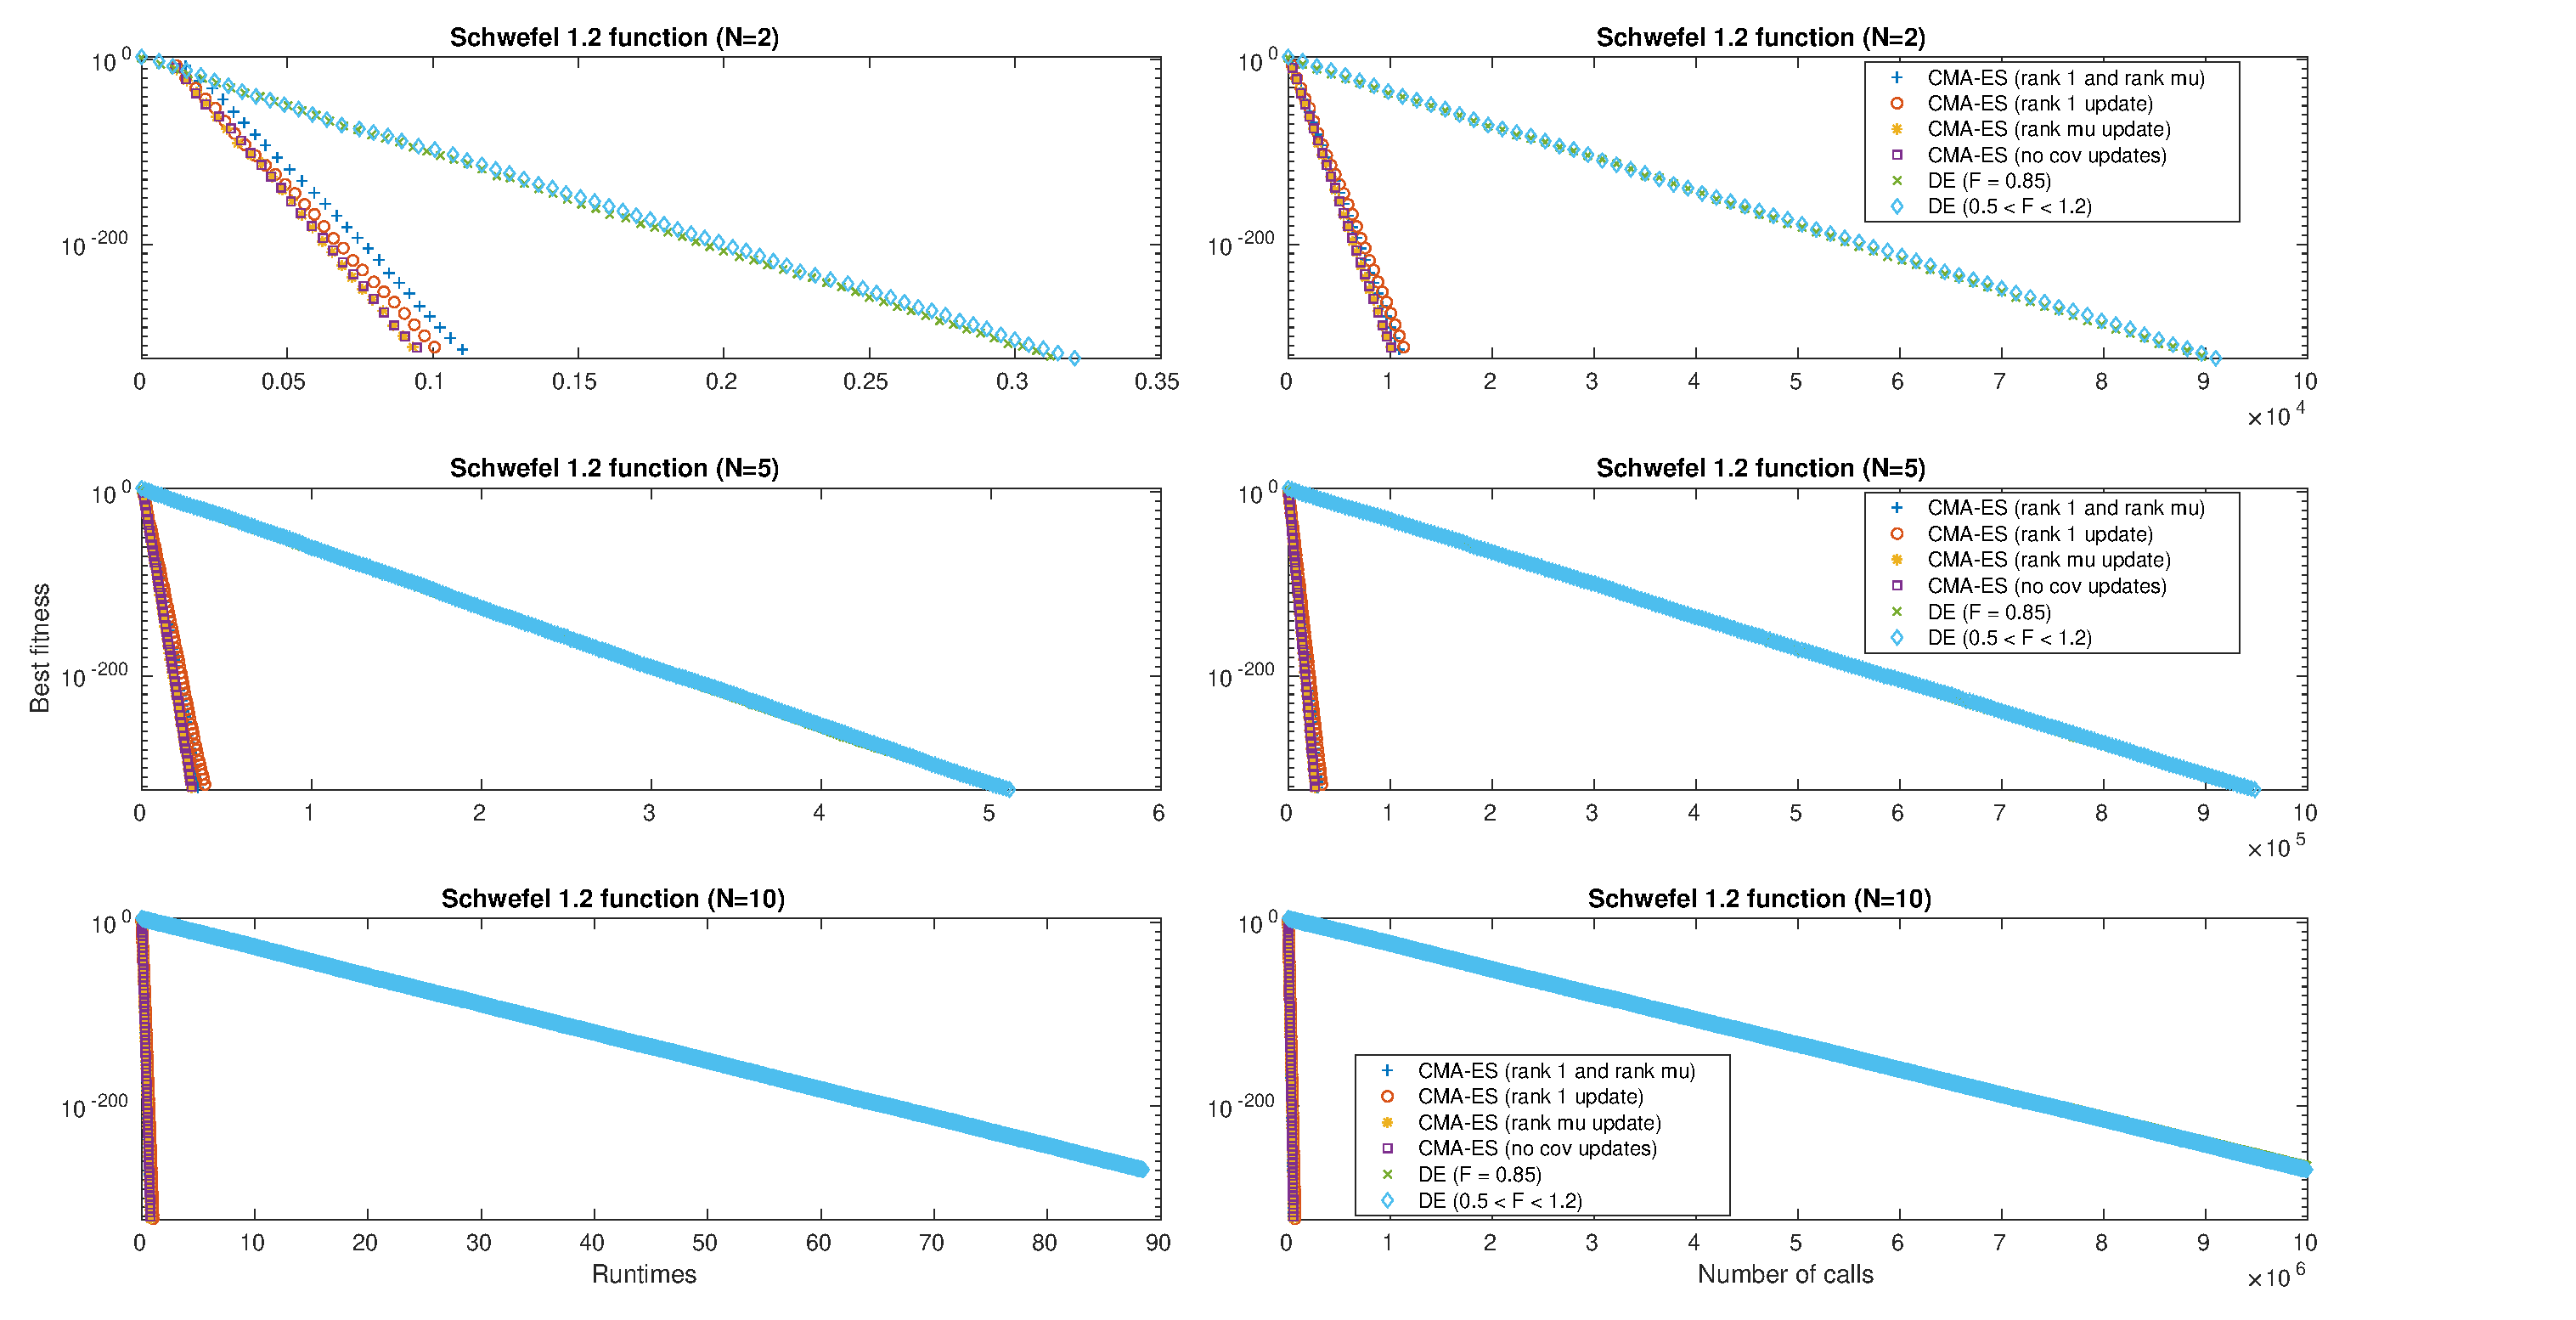
\includegraphics[width=1.5\linewidth]{pics/schwefel.eps}
        \caption{Best fitness vs. Runtimes (left column) and
        best fitness vs. Number of calls (right column)
        for the Schwefel function (N=\{2,~5,~10\})}
        \label{fig:schwefel}
    \end{figure}
\end{landscape}
% END LANDSCAPE PAGE

% BEGIN LANDSCAPE PAGE
\begin{landscape}
\thispagestyle{empty}
    \begin{figure}
        \hspace*{-4.5cm}
        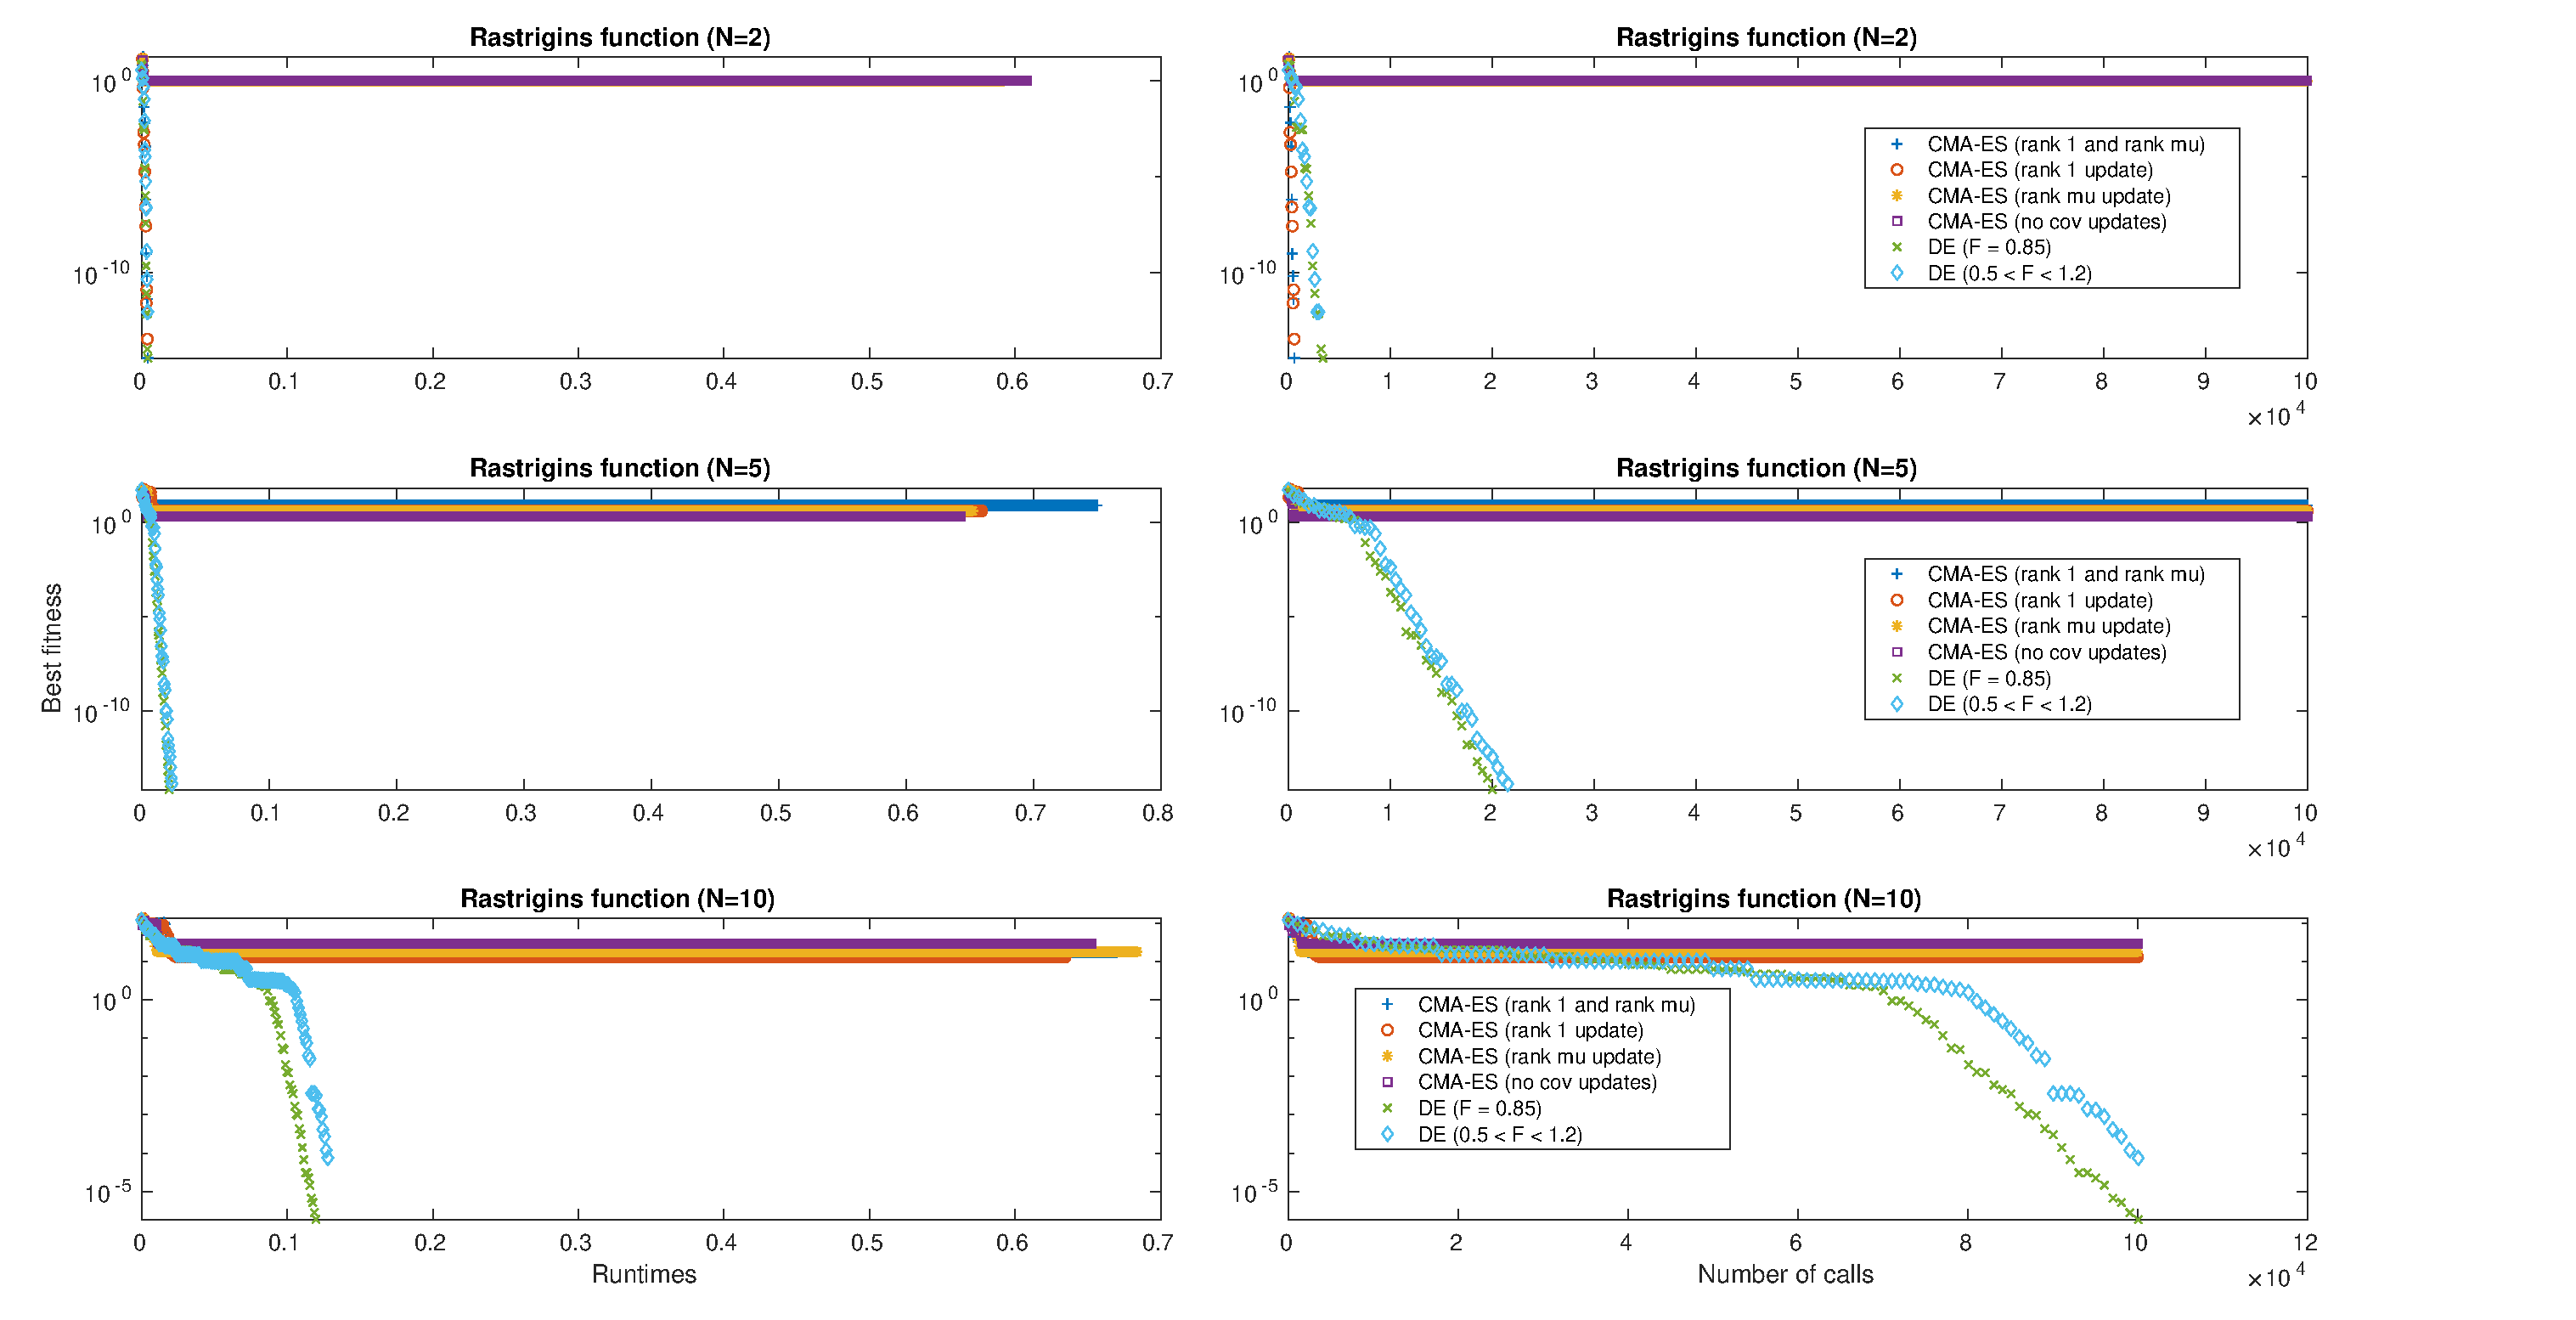
\includegraphics[width=1.5\linewidth]{pics/rastrigins.eps}
        \caption{Best fitness vs. Runtimes (left column) and
        best fitness vs. Number of calls (right column)
        for the Rastrigins function (N=\{2,~5,~10\})}
        \label{fig:rastrigin}
    \end{figure}
\end{landscape}
% END LANDSCAPE PAGE

\section{Boxplot benchmark}

In this section of the experiment the CMA-ES and DE algorithms in the spherical problem, the Schwefel problem, and Rastrigins problem are compared for $N=\{2,5,10\}$ using the boxplots of the distributions of Euclidean distances of the best individuals to the optimal values of the functions over 50 runs (for all of them $x_{\text{opt}} = \mathbf{\vec{0}}$).

From figure \ref{fig:sphere_bplot} (spherical function) we can conclude that the all variations of CMA-ES outperform all variations of DE when we increase the dimension of the space. For $N=2$, all the algorithms work similarly well and finds the answer with the precision of $10^{-162}$. Mean values and quartiles are approximately at the same level. When the dimension is increased to 5 or ten, the difference in accuracy between CMA-ES and DE gets high. CMA-ES has the precision of approx. $10^{-150}$, while DE has $~10^{-20}$.

The same situation is true for the Schwefel 1.2 function (Fig. \ref{fig:schwefel_bplot}). For low dimensions, both algorithms find accurate solutions, while CMA-ES scales better with higher dimensions.

In the Fig. \ref{fig:rastrigins_bplot} (Rastrigin's function), we see the opposite situation. CMA-ES gets stuck in local minima and is unable to find any accurate solutions. DE, on the other hand, seems to be able to escape the local optima and find better, more accurate solutions. DE still converges slowly in the $N=2$ and $N=5$ case, given $10^5$ maximum number of function evaluations, the precision is approx. $10^{-10}$, which is good. But in the case of $N=10$, the convergence is much slower and the boxplot show us the precision of $10^{-2}$, which is local optima, which means that it is still converging.

% BEGIN LANDSCAPE PAGE
\begin{landscape}
\thispagestyle{empty}
    \begin{figure}
        \hspace*{-6cm}
        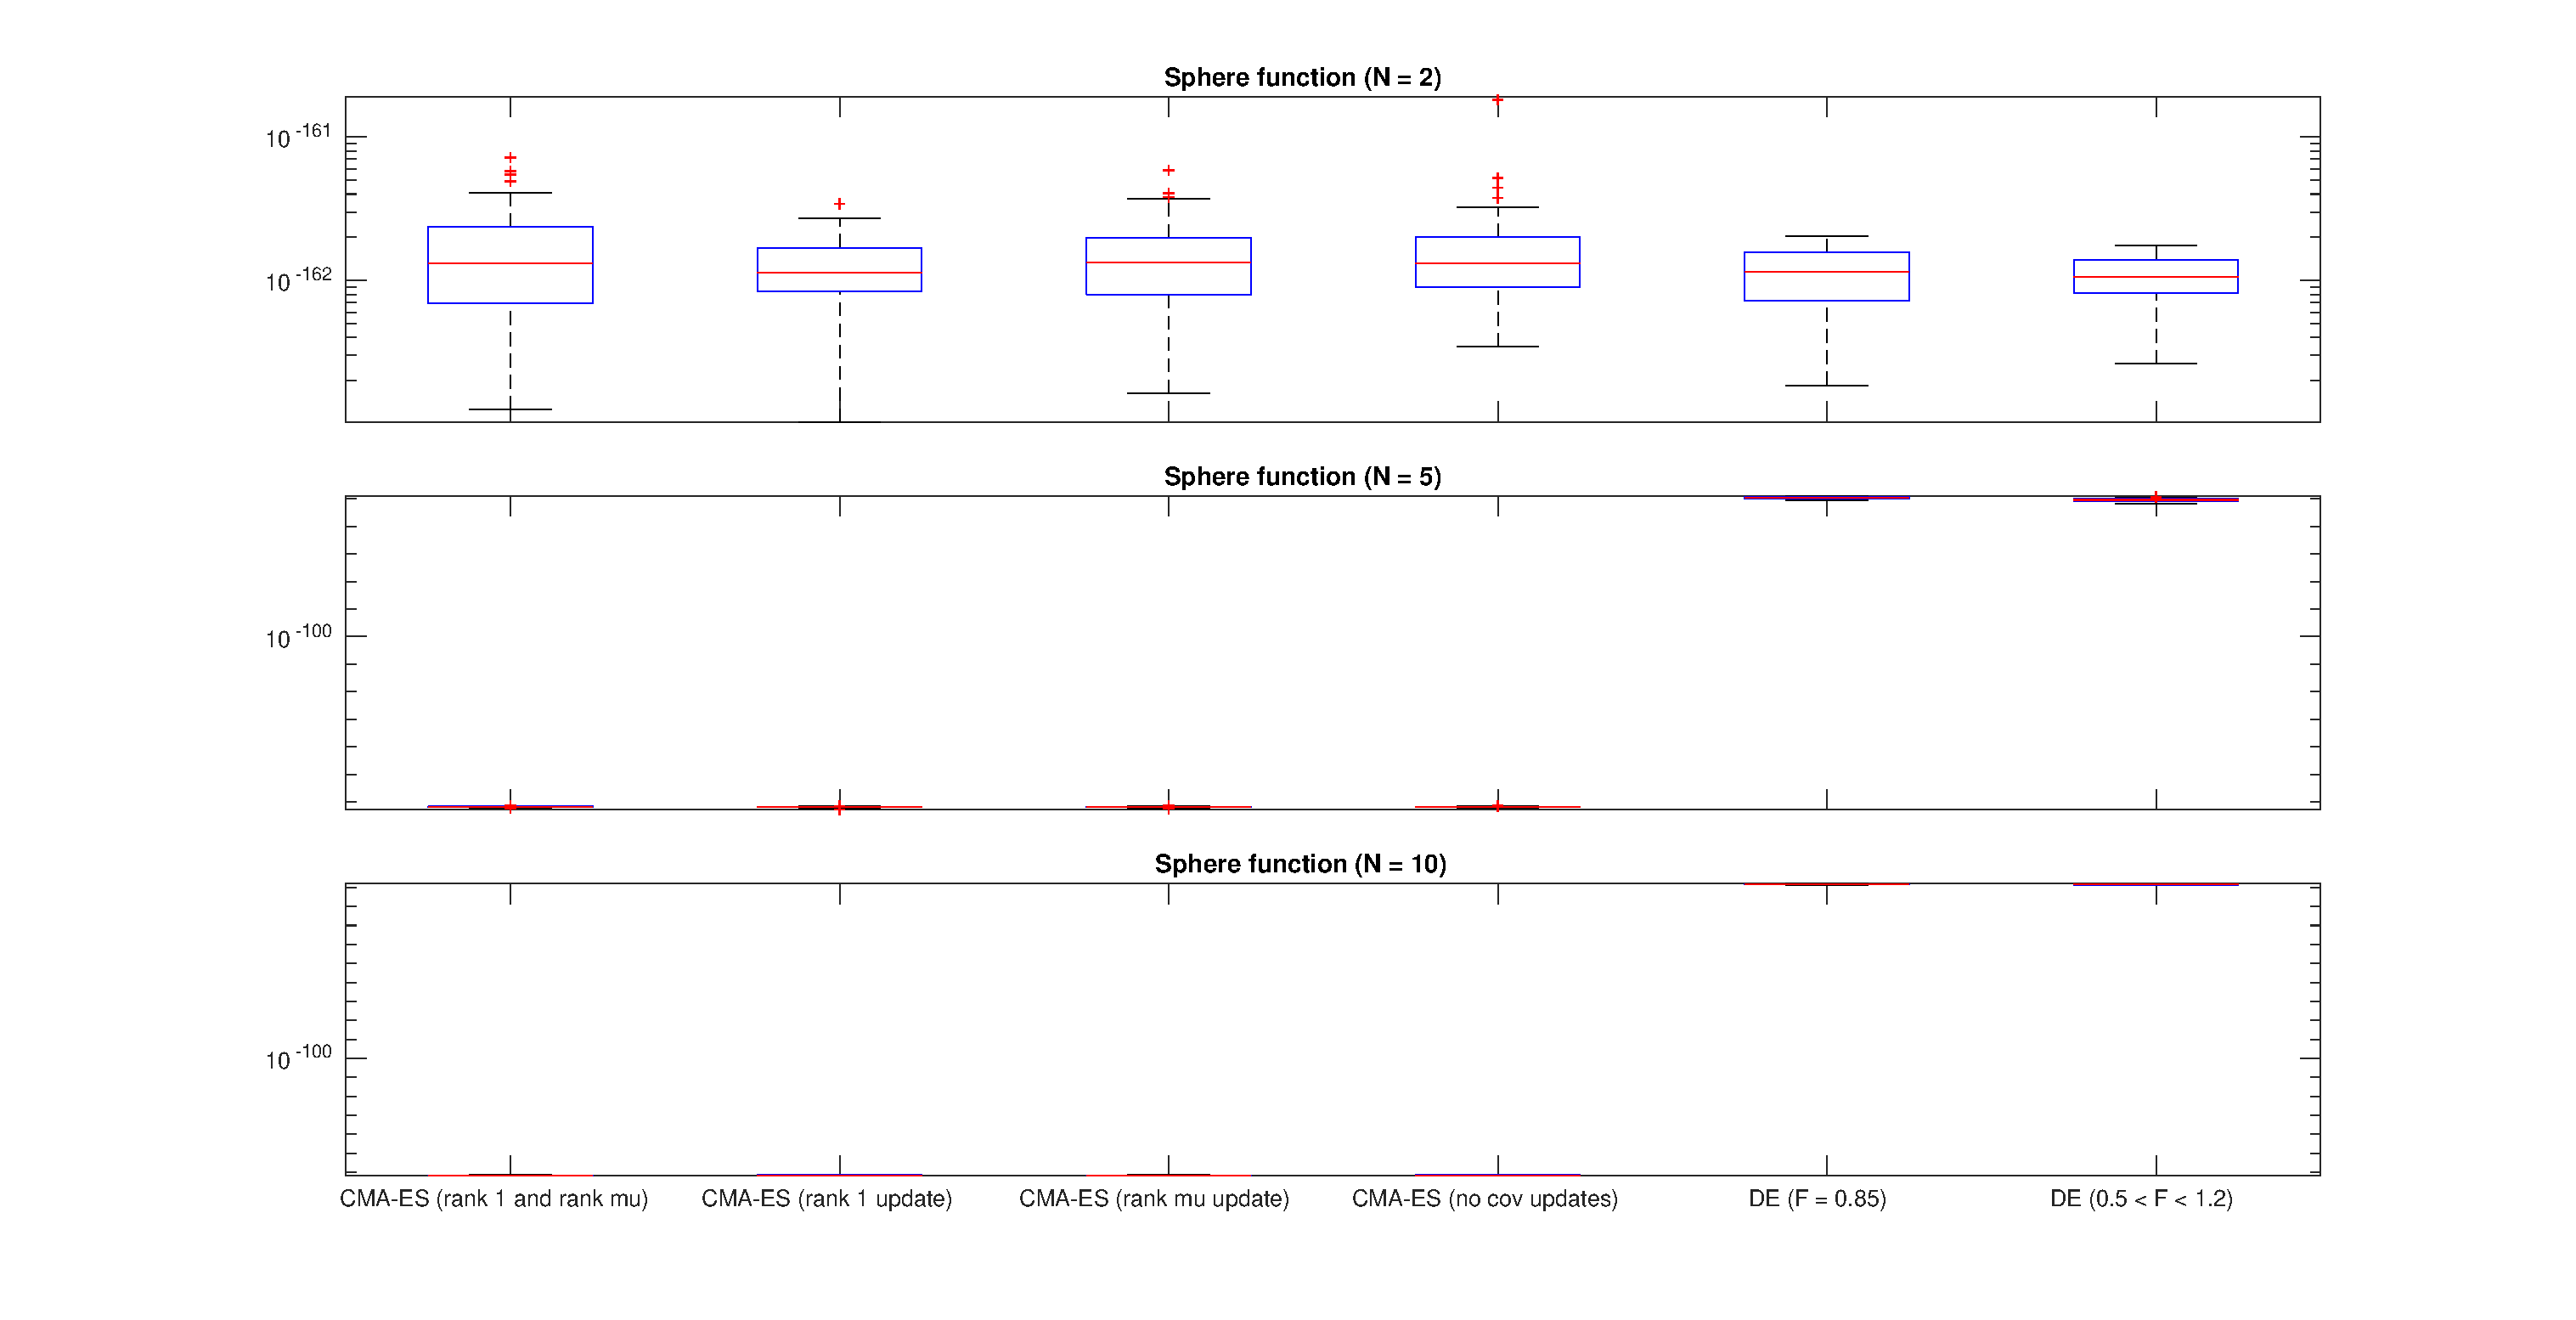
\includegraphics[width=1.5\linewidth]{pics/sphere_bplot.eps}
        \caption{Distribution of the distances of the best solution to the origin over 50 runs for spherical fitness}
        \label{fig:sphere_bplot}
    \end{figure}
\end{landscape}
% END LANDSCAPE PAGE

% BEGIN LANDSCAPE PAGE
\begin{landscape}
\thispagestyle{empty}
    \begin{figure}
        \hspace*{-6cm}
        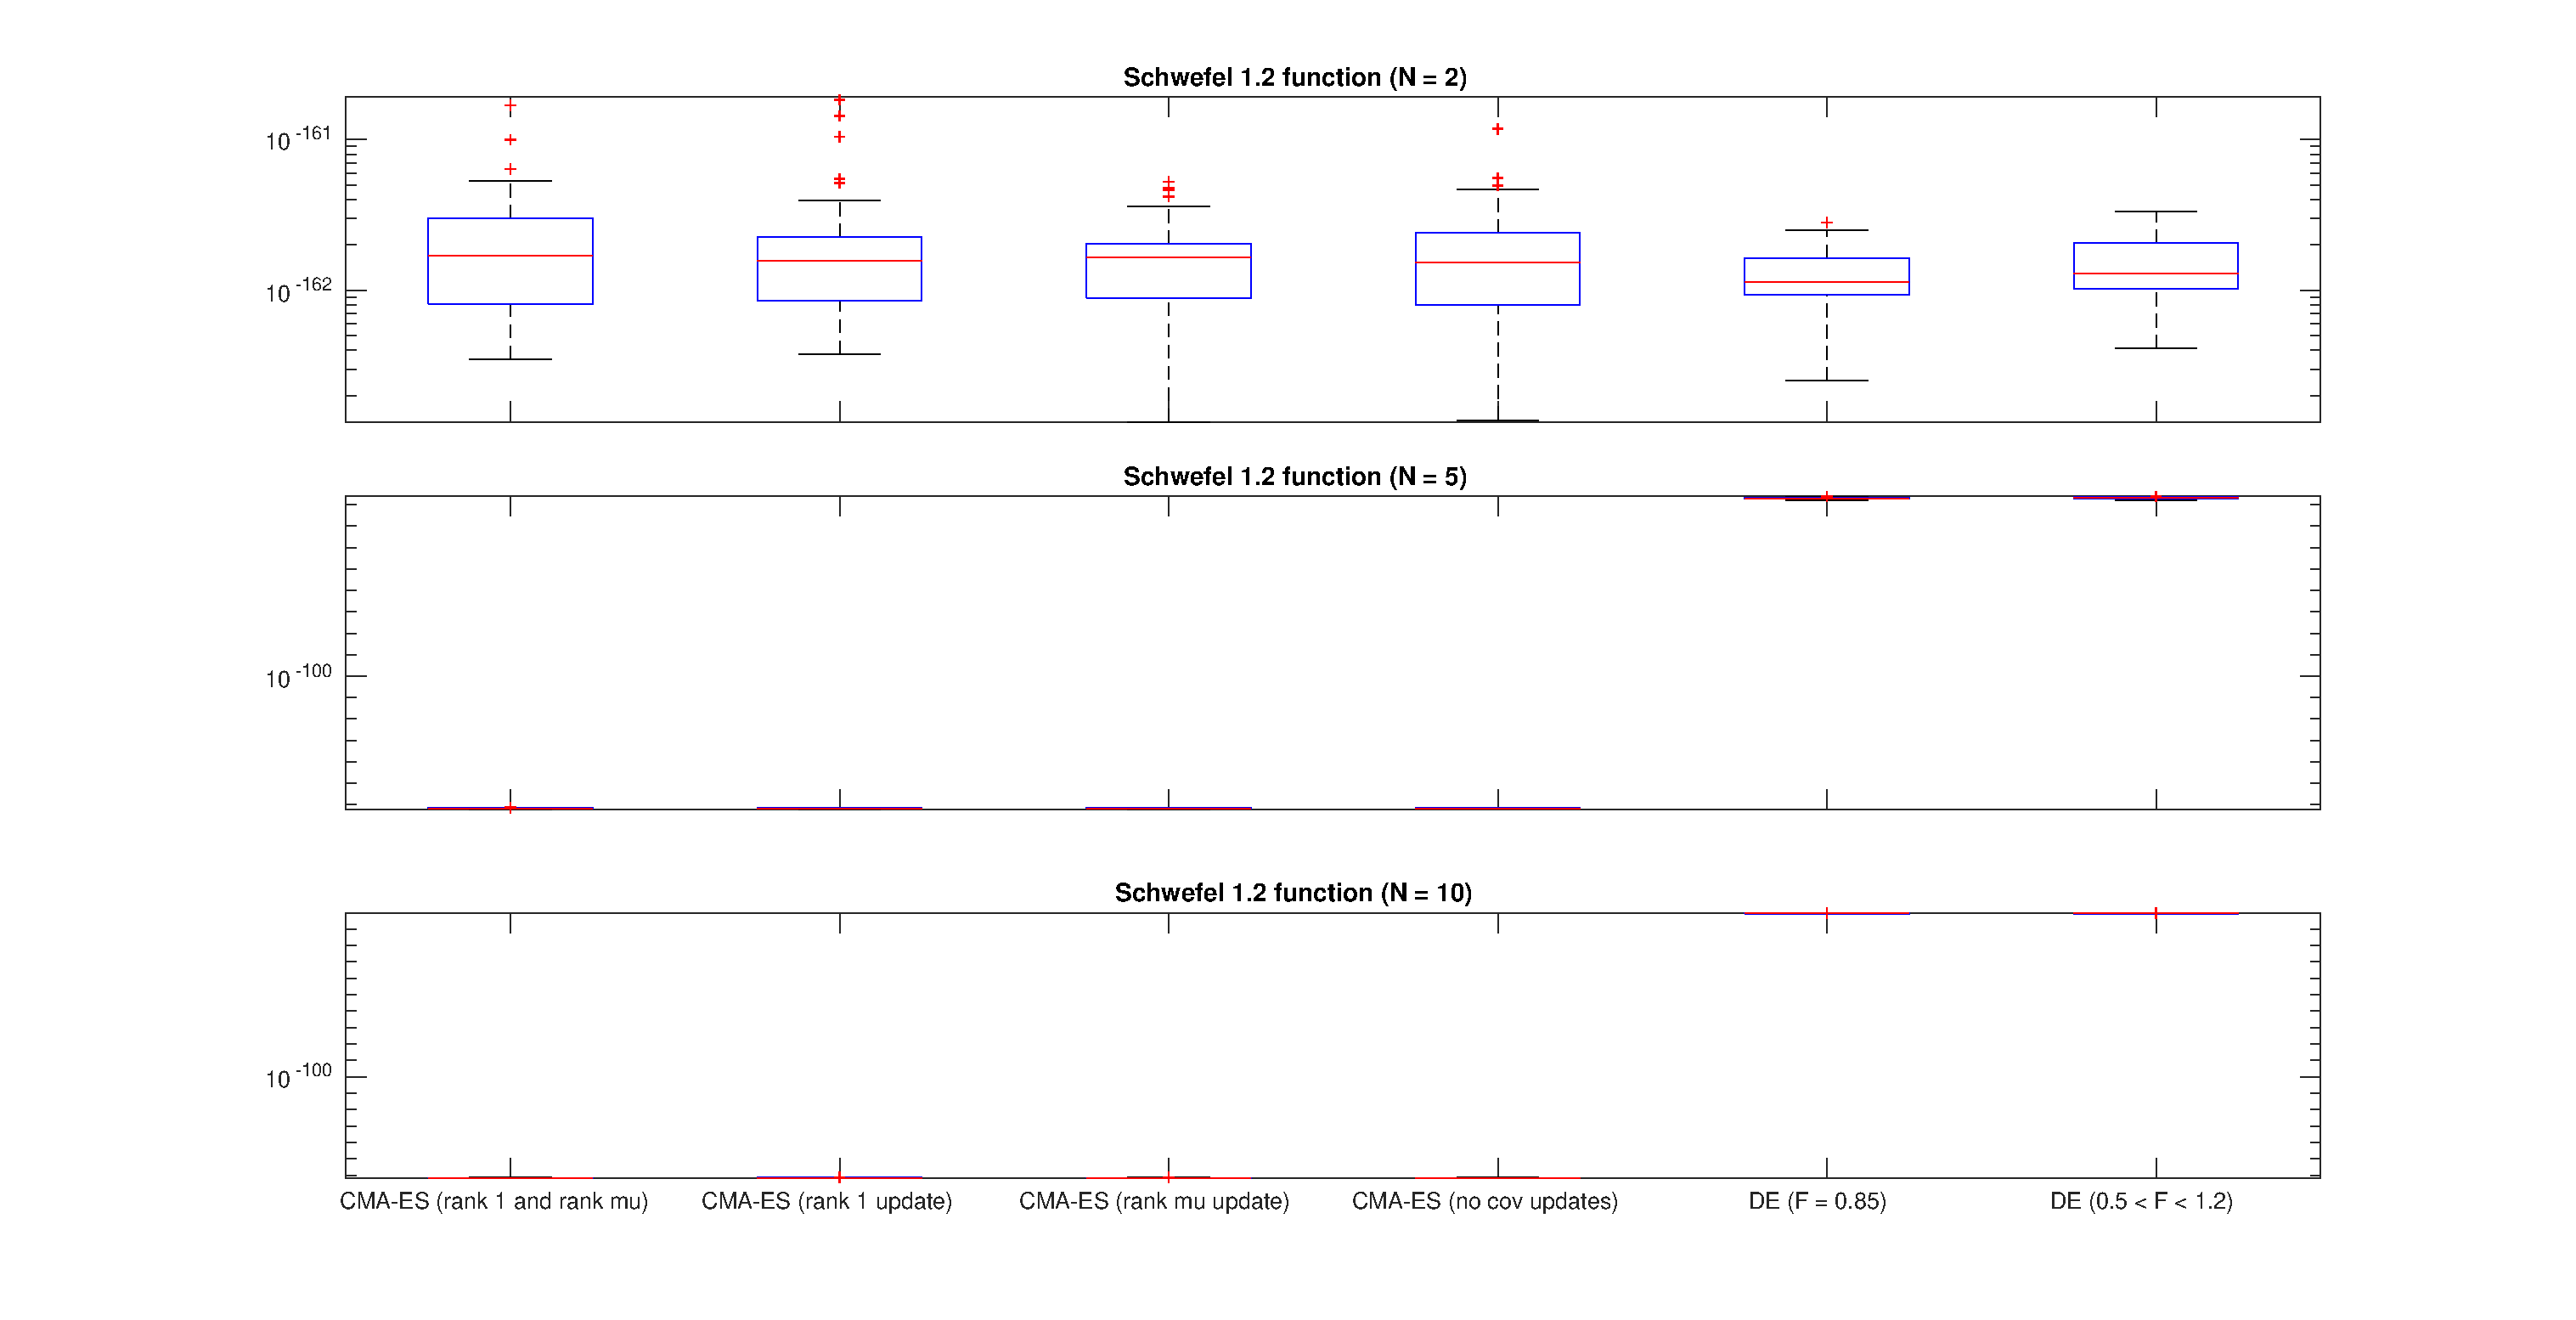
\includegraphics[width=1.5\linewidth]{pics/schwefel_bplot.eps}
        \caption{Distribution of the distances of the best solution to the origin over 50 runs for Schwefel fitness}
        \label{fig:schwefel_bplot}
    \end{figure}
\end{landscape}
% END LANDSCAPE PAGE

% BEGIN LANDSCAPE PAGE
\begin{landscape}
\thispagestyle{empty}
    \begin{figure}
        \hspace*{-6cm}
        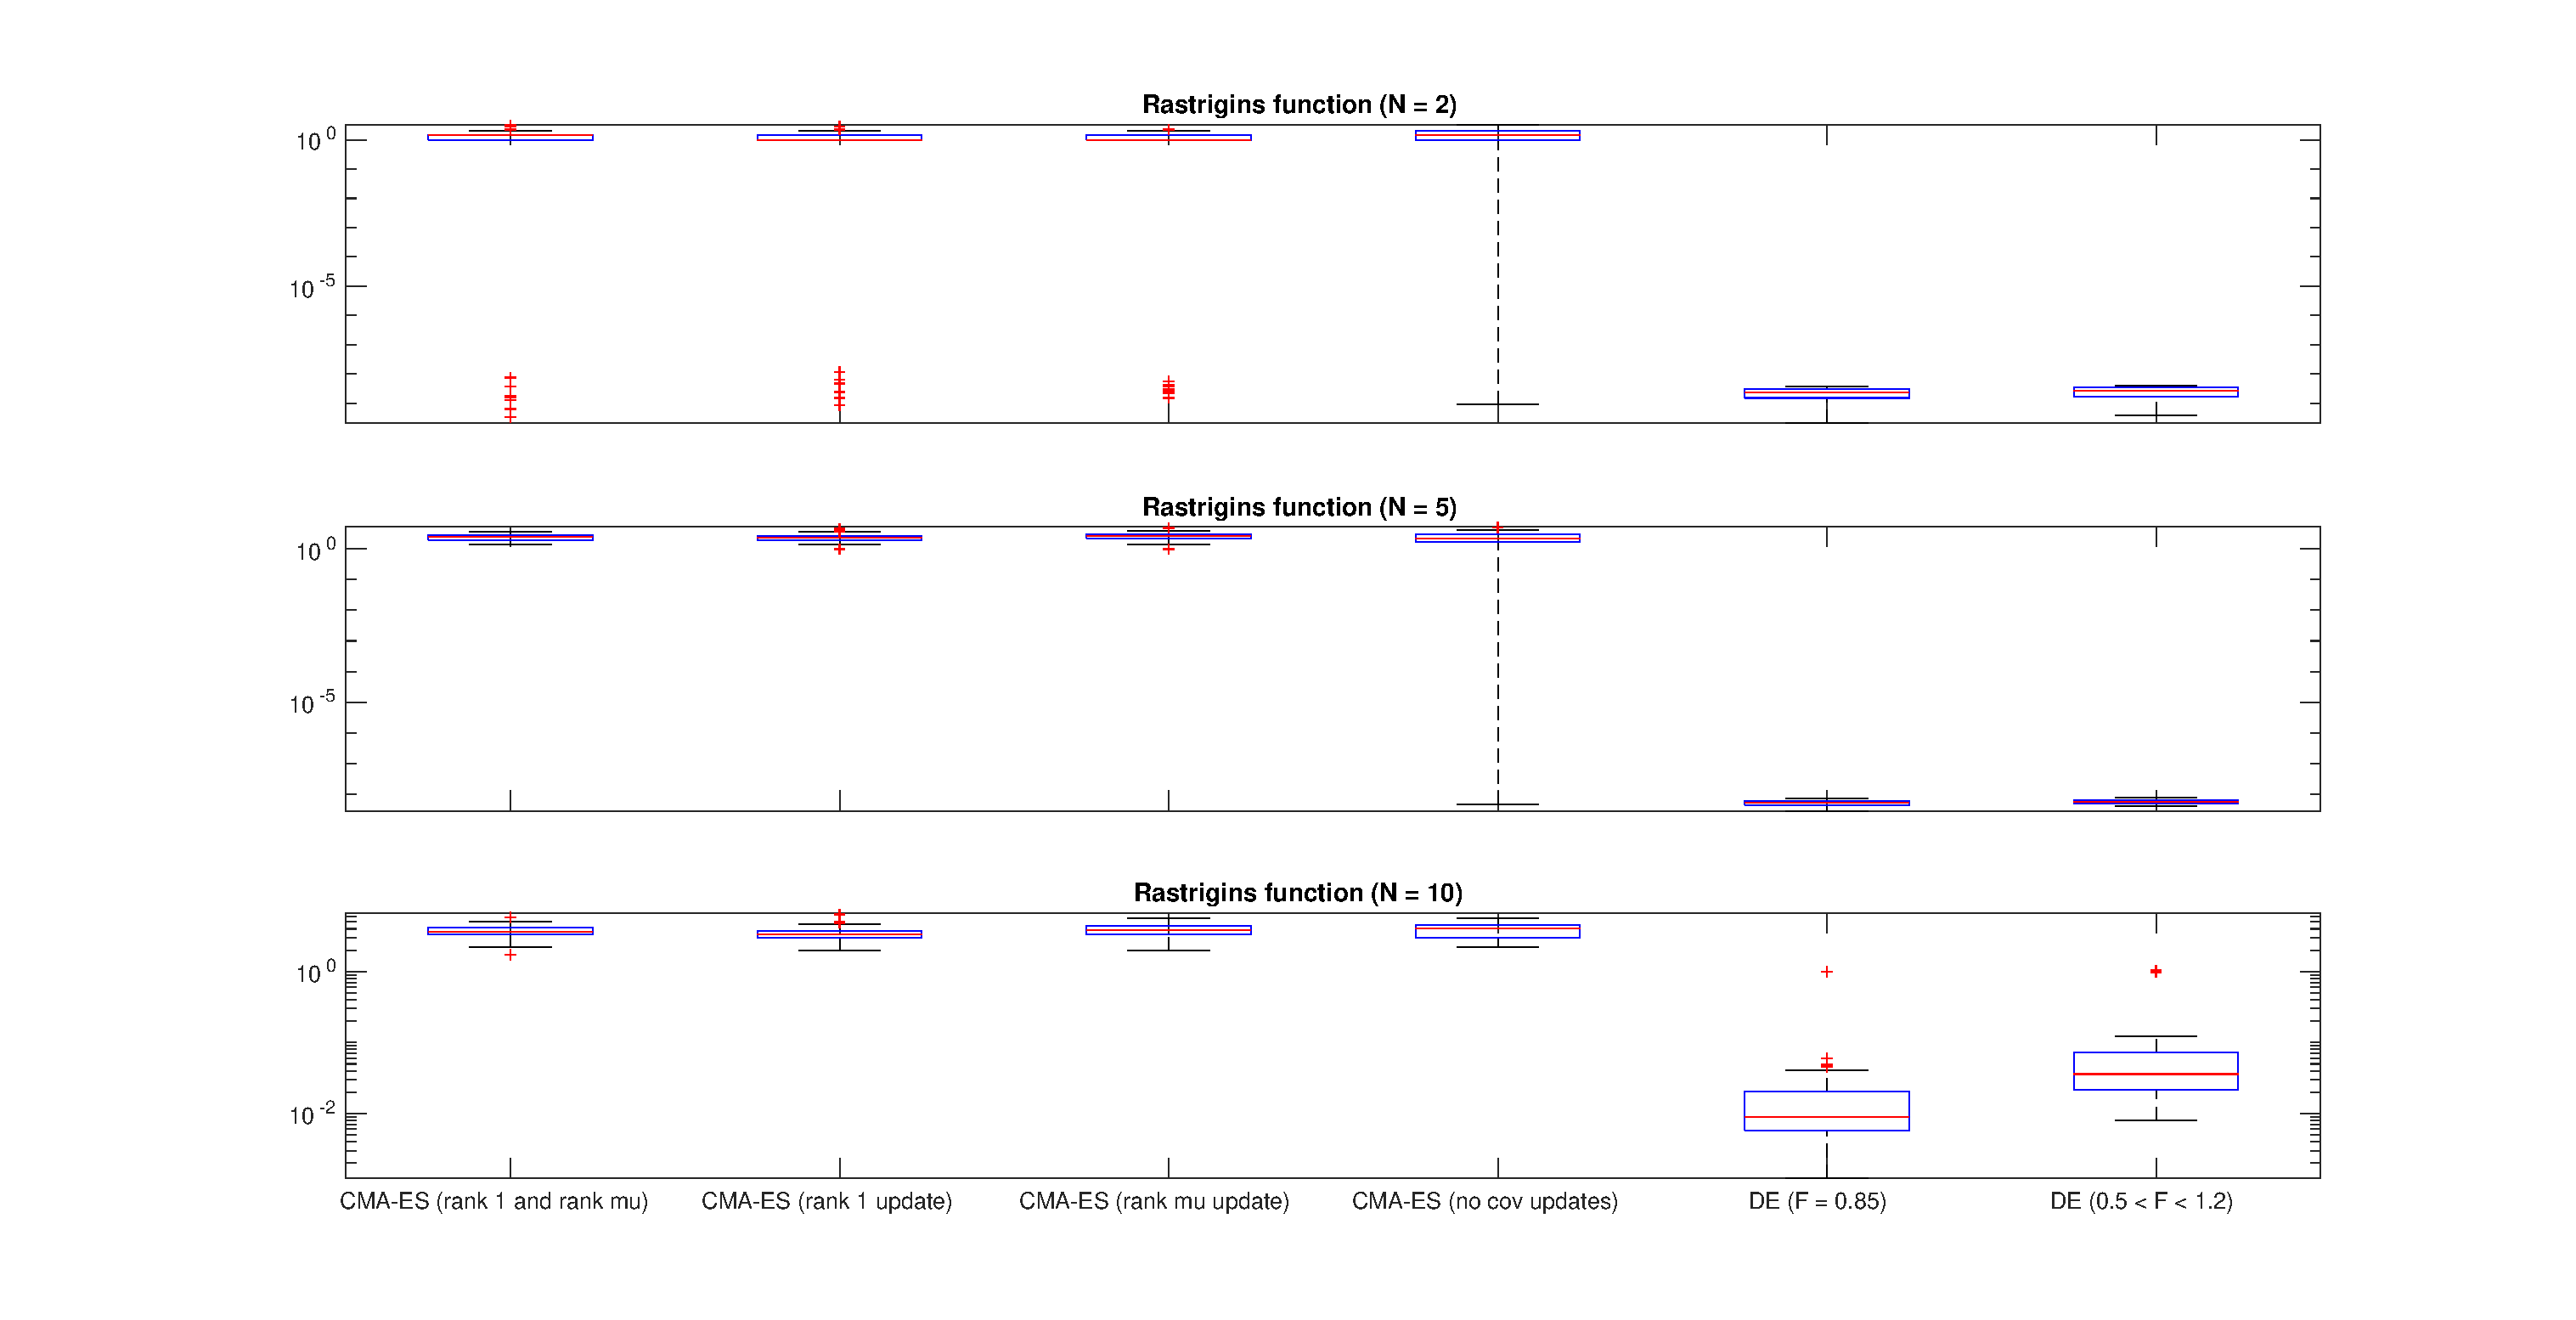
\includegraphics[width=1.5\linewidth]{pics/rastrigins_bplot.eps}
        \caption{Distribution of the distances of the best solution to the origin over 50 runs for Rastrigins fitness}
        \label{fig:rastrigins_bplot}
    \end{figure}
\end{landscape}
% END LANDSCAPE PAGE

\section{Scaling with N}
\subsection{Number of evaluations vs. dimension size}
As figures \ref{fig:sphere_nvn}, \ref{fig:schwefel_nvn}, and \ref{fig:rastrigins_nvn} show, the speed of the algorithms vary significantly with the dimensionality of the problem. Higher dimensional problems are significantly harder to solve. The algorithms were run until convergence on a suitable solution. The number of function evaluations required to find a solution was plotted against the dimension of the problem for all three problems. For all three problems, DE seems to scale exponentially with $N$ whereas CMA-ES appears to scale linearly. For Rastrigins function, we can see that CMA-ES occasionally is able to identify the solution (the strange, apparently random bumps). This is consistent with the boxplots for Rastrigins function, which has outliers with much smaller distances from the maximum.

\begin{figure}[H]
    \centering
    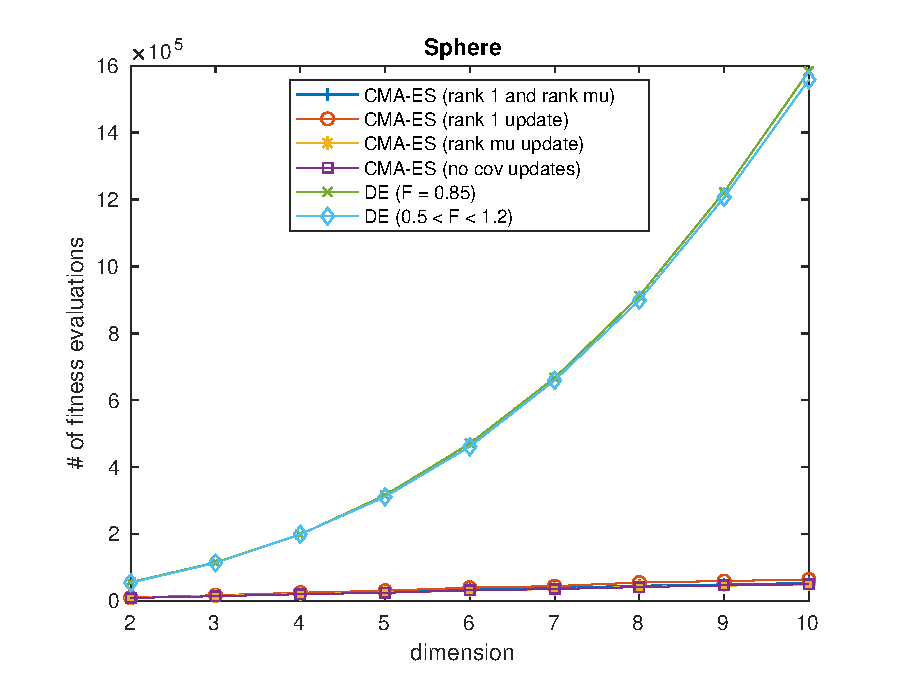
\includegraphics[width=0.8\linewidth]{pics/sphere_NvN.eps}
    \caption{Number of evaluations vs. dimension for the Sphere function}
    \label{fig:sphere_nvn}
\end{figure}

\begin{figure}[H]
    \centering
    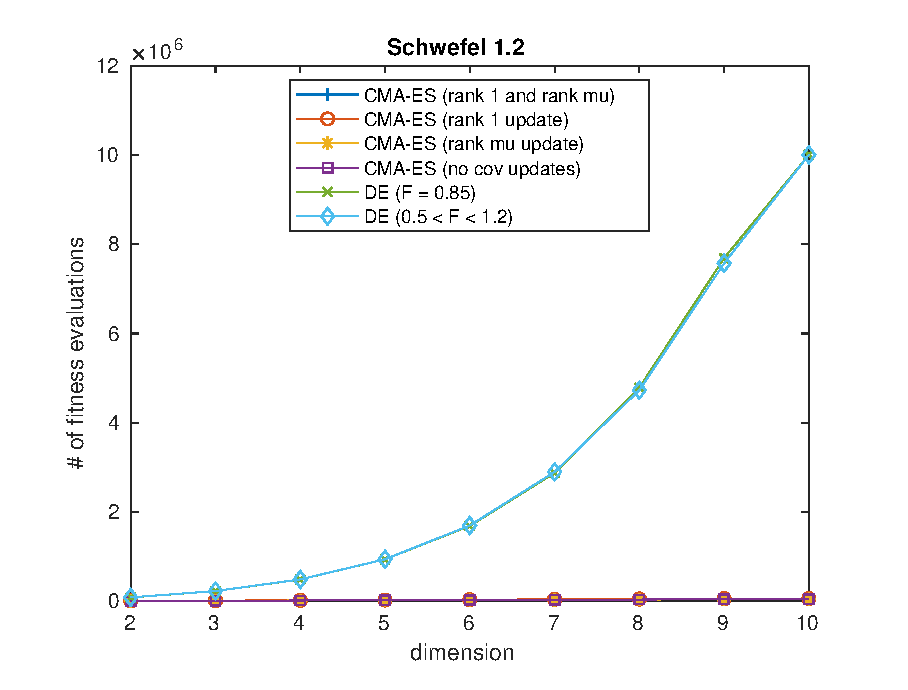
\includegraphics[width=0.75\linewidth]{pics/schwefel_NvN.eps}
    \caption{Number of evaluations vs. dimension for the Schwefel function}
    \label{fig:schwefel_nvn}
\end{figure}

\begin{figure}[H]
    \centering
    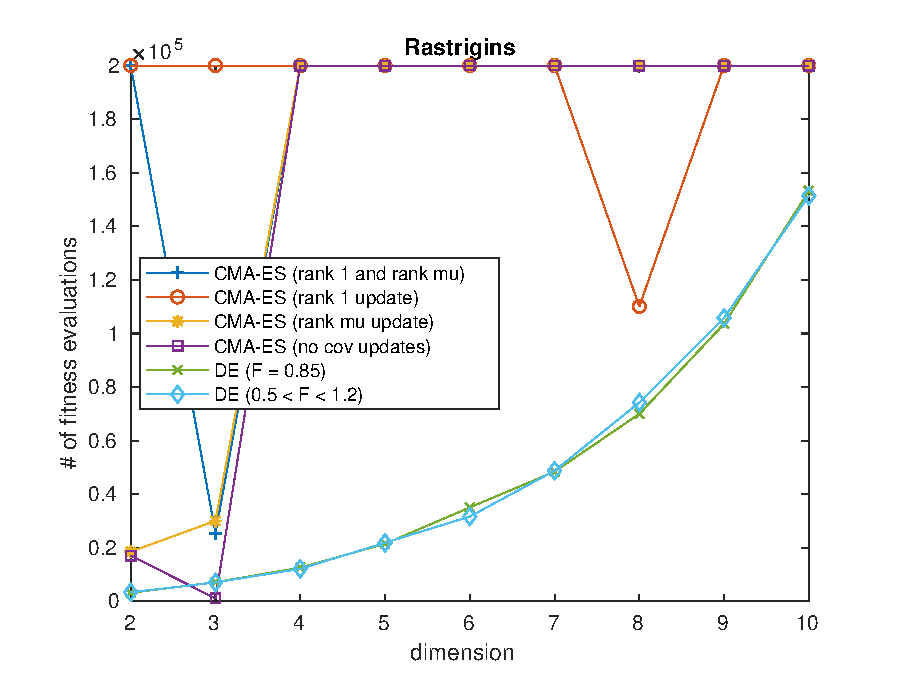
\includegraphics[width=0.75\linewidth]{pics/rastrigins_NvN.eps}
    \caption{Number of evaluations vs. dimension for the Rastrigin's function}
    \label{fig:rastrigins_nvn}
\end{figure}

\subsection{Runtimes vs. dimension size}
Figures \ref{fig:sphere_tvn}, \ref{fig:schwefel_tvn}, and \ref{fig:rastrigins_tvn} show the runtime of the algorithms plotted against the dimension of the problem. DE runs significantly faster than CMA-ES for all three problems. Interestingly, it seems that the runtimes of DE algorithms do not vary significantly with $N$ for the sphere and Rastrigins. 

\begin{figure}[H]
    \centering
    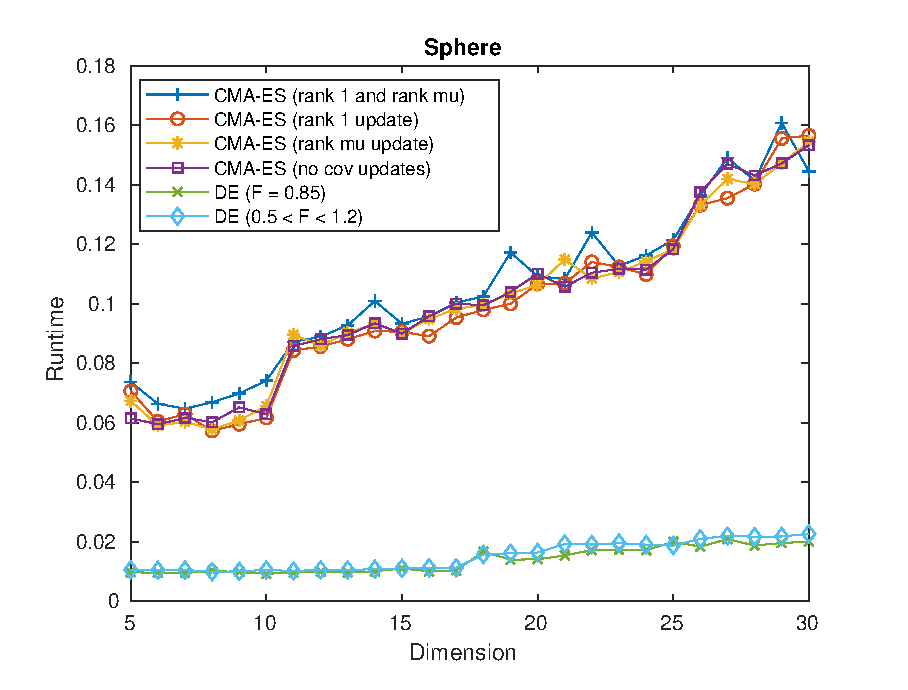
\includegraphics[width=0.8\linewidth]{pics/sphere_TvN.eps}
    \caption{Runtime vs. dimension for the Sphere function}
    \label{fig:sphere_tvn}
\end{figure}

\begin{figure}[H]
    \centering
    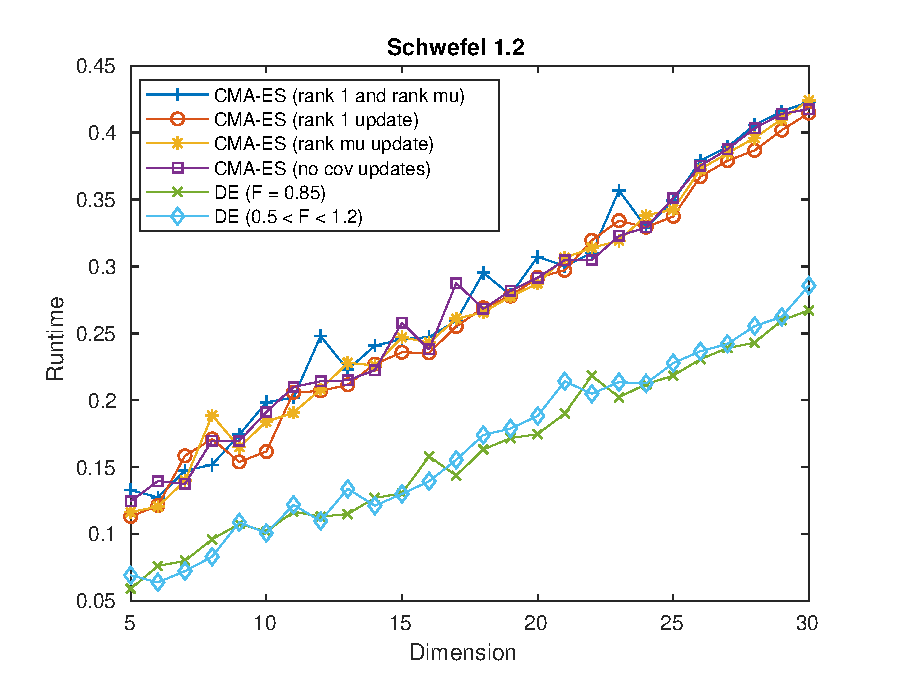
\includegraphics[width=0.75\linewidth]{pics/schwefel_TvN.eps}
    \caption{Runtime vs. dimension for the Schwefel function}
    \label{fig:schwefel_tvn}
\end{figure}

\begin{figure}[H]
    \centering
    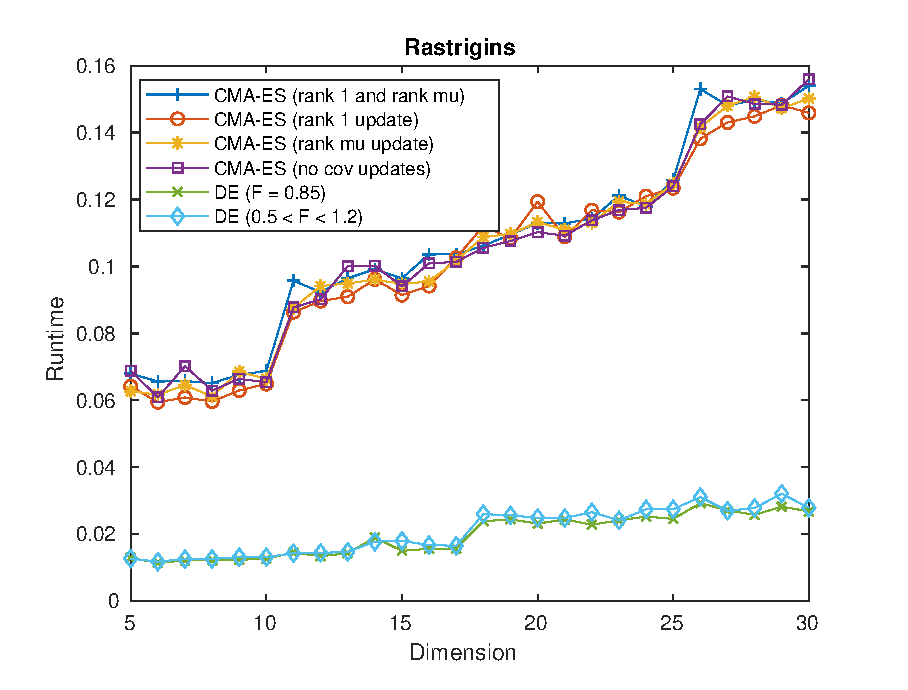
\includegraphics[width=0.75\linewidth]{pics/rastrigins_TvN.eps}
    \caption{Runtime vs. dimension for the Rastrigin's function}
    \label{fig:rastrigins_tvn}
\end{figure}



\section{Conclusion}
Overall, DE finds solutions in all three cases, but the precision is not high. CMA-ES converges very quickly to whatever optima it can, be it global or local. All algorithms are stable in finding some optima, as quartiles in the boxplots are relatively close to the mean. That is, deviation is small. 

Additionally to these benchmarks, it may be interesting to test these algorithms for fitness landscapes with local optima very close to each other, to see if CMA-ES is able to 'jump' across sufficiently short distances in the fitness landscape. Similarly, fitness landscapes with local optima very far apart could demonstrate how good DE is at navigating these types of landscapes. Visualizing the progression of individuals in the DE algorithm may also help illustrate how it is able to escape from local optima.




\end{document}
